\documentclass[12pt]{report}
\usepackage[utf8]{inputenc}
\usepackage[english]{babel}
\usepackage[T1]{fontenc}
\usepackage{graphicx, color}
\usepackage{float}
\usepackage{subcaption}
\usepackage[a4paper,margin=2cm]{geometry}
\usepackage[authoryear]{natbib}
%\usepackage{refcheck}
\usepackage{hyperref}
\hypersetup{
    colorlinks,
    citecolor=black,
    filecolor=black,
    linkcolor=black,
    urlcolor=black
}

\begin{document}

\begin{titlepage}

\newcommand{\HRule}{\rule{\linewidth}{0.5mm}} % Defines a new command for the horizontal lines, change thickness here
\center % Center everything on the page
 
%----------------------------------------------------------------------------------------
%	HEADING SECTIONS
%----------------------------------------------------------------------------------------


\includegraphics[width=\linewidth]{assets/logos/uvaENG.eps}\\[2.5cm]
\textsc{\Large MSc Artificial Intelligence}\\[0.2cm]
\textsc{\Large Master Thesis}\\[0.5cm]

%----------------------------------------------------------------------------------------
%	TITLE SECTION
%----------------------------------------------------------------------------------------

\HRule \\[0.4cm]
{ \huge \bfseries Detecting and Addressing Change in Machine Learning Data Pipelines}\\[0.4cm] % Title of your document
\HRule \\[0.5cm]
 
%----------------------------------------------------------------------------------------
%	AUTHOR SECTION
%----------------------------------------------------------------------------------------

by\\[0.2cm]
\textsc{\Large Bogdan Floris}\\[0.2cm] %you name
12140910\\[1cm]


%----------------------------------------------------------------------------------------
%	DATE SECTION
%----------------------------------------------------------------------------------------

{\Large \today}\\[1cm] % Date, change the \today to a set date if you want to be precise

Number of credits: 48 ECTS\\ %
November 2019 - July 2020\\[1cm]%

%----------------------------------------------------------------------------------------
%	COMMITTEE SECTION
%----------------------------------------------------------------------------------------
\noindent
\begin{minipage}[t]{0.4\textwidth}
\begin{flushleft} \large
\emph{Supervisors:} \\
prof. dr. Paul \textsc{Groth}\\
dr. Jakub \textsc{Zavrel}
\end{flushleft}
\end{minipage}
\begin{minipage}[t]{0.4\textwidth}
\begin{flushright} \large
\emph{Assessor:} \\
prof. dr. Paul \textsc{Groth}\\
\end{flushright}
\end{minipage}\\[2cm]

%----------------------------------------------------------------------------------------
%	LOGO SECTION
%----------------------------------------------------------------------------------------

%\framebox{\rule{0pt}{2.5cm}\rule{2.5cm}{0pt}}\\[0.5cm]
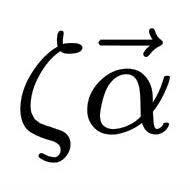
\includegraphics[width=2.5cm]{assets/logos/zeta-alpha-logo.jpg}\\ % Include a department/university logo - this will require the graphicx package
\textsc{\large Zeta Alpha Vector}\\[1.0cm] % 
 
%----------------------------------------------------------------------------------------

\vfill % Fill the rest of the page with whitespace

\end{titlepage}

\chapter*{Abstract}

Insert abstract here.

\chapter*{Acknowledgements}

Insert the acknowledgements here.

\tableofcontents

\listoffigures

\listoftables

\chapter{Introduction}

\begin{itemize}
    \item General introduction to the field (Machine Learning, NLP)
    \item Small overview of the topic being researched in this paper
    \item Why this topic?
    \item Description of the framework \ref{fig:framework}
\end{itemize}

\begin{figure}[h!]
\centering
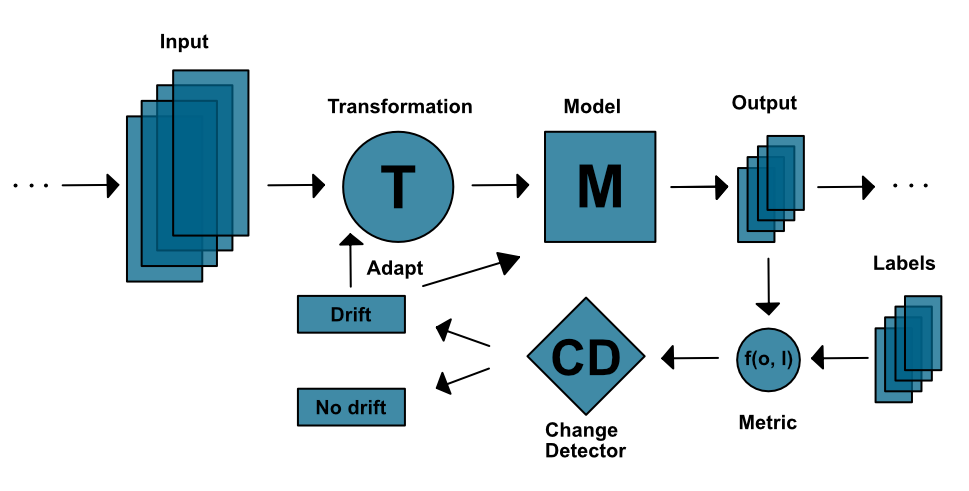
\includegraphics[width=\linewidth]{assets/introduction/framework.png}
\caption{General overview of the architecture}
\label{fig:framework}
\end{figure}

Random citation to check that the references are shown: \citep{Heng_Wang_2015}.

\section{Research Questions}

The main goal of this thesis is to develop a general framework in which machine learning models that are part of streaming data pipelines can detect changes in their output distribution and adapt to them accordingly, while also successfully applying this framework on a specific natural language processing use case that is of interest to Zeta Alpha Vector. This comprehensive topic will be tackled with the following research questions, covered below together with a short description for each question.

\paragraph*{How can we quickly detect that the output distribution of a model has changed given a continuous stream of data, and then report on the degree of change?} Insert description of this research question

\paragraph*{Given that a change was detected, how can we adapt the model efficiently such that the performance is the same as it previously was before the change?} Insert overall description of the question here, them break it down to the two other questions:
\begin{itemize}
    \item \textbf{Given a small change (gradual drift or small abrupt drift), can we adapt the model by feeding it with a few examples, compared to retraining it from scratch?} Description about this subquestion.
    \item \textbf{Given a big change (big abrupt drift), can we adapt the model by finding a mapping between the old outputs and the new ones which is less expensive to compute than retraining the model from scratch?} Description about this subquestion
\end{itemize}

\chapter{Background}

\section{Streaming Data Pipelines and Online Learning}

\begin{itemize}
    \item Explain what streams of data are and how data pipelines are more common in an industry setting
    \item Difference between online learning and traditional batch learning, and argue its pros and cons
\end{itemize}

\section{Concept drift}

\begin{itemize}
    \item Explain what concept drift is in theory
    \item Explain the different types of concept drift that are relevant for this thesis with references to the figures
    \item Explain how the concept will be used in this thesis and how it is a bit different from how it is used in practice
\end{itemize}

\begin{figure}[ht!]
\centering
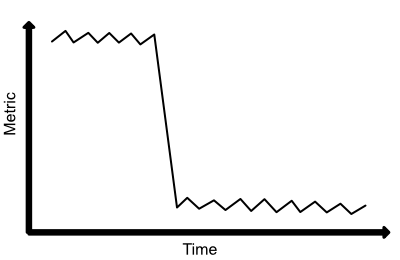
\includegraphics[width=0.6\linewidth]{assets/preliminaries/big-abrupt-drift.png}
\caption{Big abrupt concept drift}
\label{fig:big-abrupt-drift}
\end{figure}

\begin{figure}[ht!]
\centering
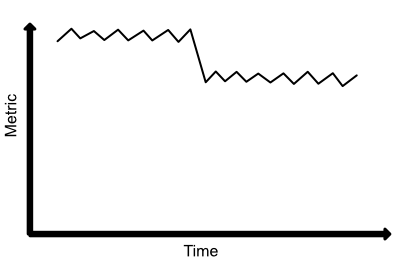
\includegraphics[width=0.6\linewidth]{assets/preliminaries/small-abrupt-drift.png}
\caption{Small abrupt concept drift}
\label{fig:small-abrupt-drift}
\end{figure}

\begin{figure}[ht!]
\centering
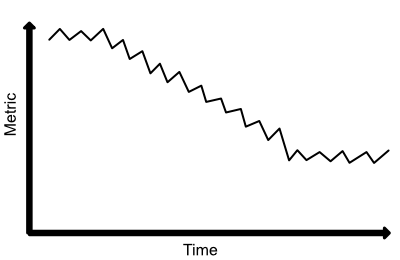
\includegraphics[width=0.6\linewidth]{assets/preliminaries/gradual-drift.png}
\caption{Gradual concept drift}
\label{fig:gradual-drift}
\end{figure}

\section{Word embeddings}

\begin{itemize}
    \item Explain word embeddings in general
    \item Focus on contextualized word embeddings
    \item Explain how they work as constants in the framework, and how changing them can affect the downstream models
\end{itemize}

\chapter{Framework}

\section{Dataset}

\subsection{The Web of Science}

Short introduction to the Web of Science and why it's good to use because of the work done by Zeta Alpha.

\begin{figure}[ht!]
\centering
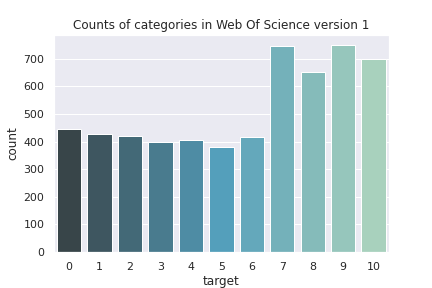
\includegraphics[width=0.8\linewidth]{assets/framework/wos_counts_1.png}
\caption{Web of Science counts for each label}
\label{fig:wos-1}
\end{figure}

Potentially add the two other variants of the Web of Science, but experiments need to be performed with those versions of the Web of Science too. That might not be worth it because analyzing the performance of the LSTM on the Web of Science is not the purpose of this thesis.

\subsection{Data stream}

Explain how the Web of Science was transformed into a data stream (batch sizes, adjustments, parameters, etc.).

\section{Models}

\subsection{Naive Bayes baseline}

\begin{itemize}
    \item Short introduction to the Naive Bayes model in general.
    \item Explain how the Naive Bayes model was adapted for our use case (things like picking the maximum over the sequence length axis in order to get a useable dataset for the model).
    \item Analyze the performance of the model and explain how the model is not robust enough.
\end{itemize}

\begin{figure}[ht!]
\centering
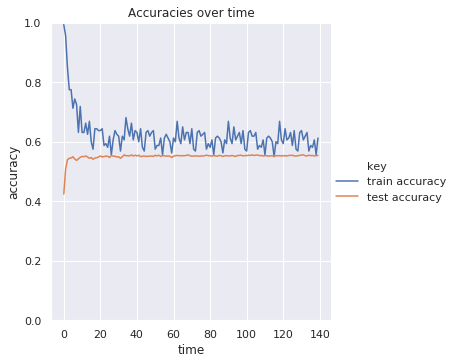
\includegraphics[width=0.8\linewidth]{assets/framework/nb_BERT_accuracy_holdout.png}
\caption{Naive Bayes accuracy over time using BERT embeddings}
\label{fig:nb-acc}
\end{figure}

Also show that the other metrics are performing on par with the accuracy for the test set using the following picture \ref{fig:nb-metrics}.

\begin{figure}[H]
\centering
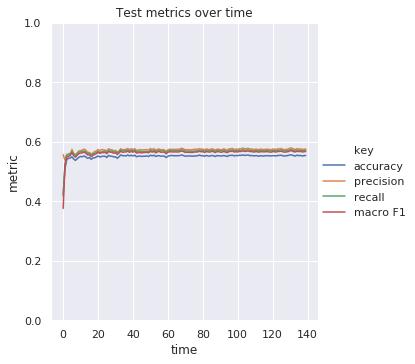
\includegraphics[width=0.8\linewidth]{assets/framework/nb_BERT_test_metrics_holdout.png}
\caption{Naive Bayes metrics over time for the test set}
\label{fig:nb-metrics}
\end{figure}

\subsection{LSTM}

\begin{itemize}
    \item Short introduction to LSTM models in general.
    \item Again, explanation of design choices made (how we solved the different sized sequences problem, and how we solved feeding it into a final fully connected layer for classification).
    \item Analyze the performance of the model and explain how the model is robust.
    \item Differences between the LSTM model and Naive Bayes one.
\end{itemize}

\begin{figure}[H]
\centering
\begin{subfigure}{.5\textwidth}
  \centering
  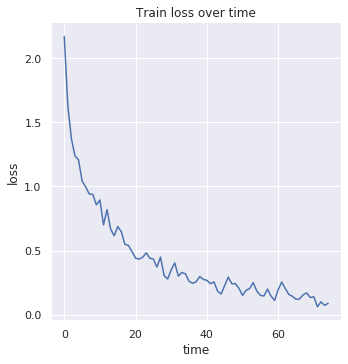
\includegraphics[width=.76\linewidth]{assets/framework/lstm_BERT_loss_holdout.png}
  \caption{Loss over time}
  \label{fig:lstm-loss}
\end{subfigure}%
\begin{subfigure}{.5\textwidth}
  \centering
  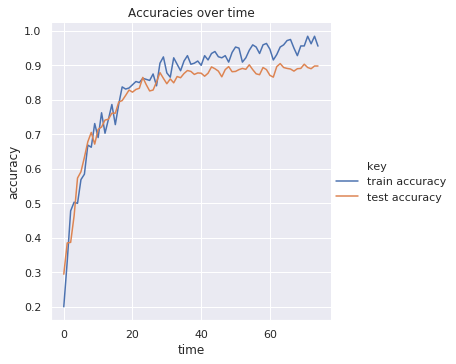
\includegraphics[width=\linewidth]{assets/framework/lstm_BERT_accuracy_holdout.png}
  \caption{Accuracy over time}
  \label{fig:lstm-acc}
\end{subfigure}
\caption{LSTM loss and accuracy over time using BERT embeddings}
\label{fig:lstm-loss-acc}
\end{figure}

Also show that the other metrics are performing on par with the accuracy for the test set using the following picture \ref{fig:lstm-metrics}.

\begin{figure}[H]
\centering
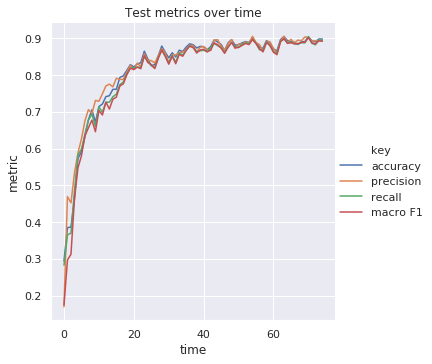
\includegraphics[width=0.8\linewidth]{assets/framework/lstm_BERT_test_metrics_holdout.png}
\caption{LSTM metrics over time for the test set}
\label{fig:lstm-metrics}
\end{figure}

\chapter{Detecting change}

\section{Experimental Setup}

\begin{itemize}
    \item Explain the different types of change detectors and their pros and cons.
    \item Explain how the experiments will be conducted: running a first stream using the embeddings that the model was trained while feeding the metrics to the change detector, then running another stream transformed using other embeddings and seeing how the model and the change detector react.
    \item We can change embeddings to produce a very small abrupt drift and change embeddings to produce a big abrupt drift.
    \item Testing for gradual drift will be done by adding random noise to the embeddings over time.
    \item Experiments will be run for both the Naive Bayes model and the LSTM model.
    \item We also need to differentiate between supervised computation of the metrics and unsupervised computation of the metrics.
    \item Mention how the sensitivity of the change detector needs to be adjusted for the unsupervised case.
    \item Mention that we show that the accuracy is 1 for the unsupervised trained model, but in practice we introduce randoms betwwen 0.9 and 1.
\end{itemize}

\section{Results}

This section will show the results for the change detection chapter without discussing the results.

\subsection{Naive Bayes model}

First show the results of changing embeddings. First BERT-DISTILBERT trying to provoke just a small abrupt drift, and then BERT-SCIBERT to provoke a big abrupt drift. We will show the supervised and the unsupervised side by side. Also explain the figures.

\begin{figure}[H]
\centering
\begin{subfigure}{.5\textwidth}
  \centering
  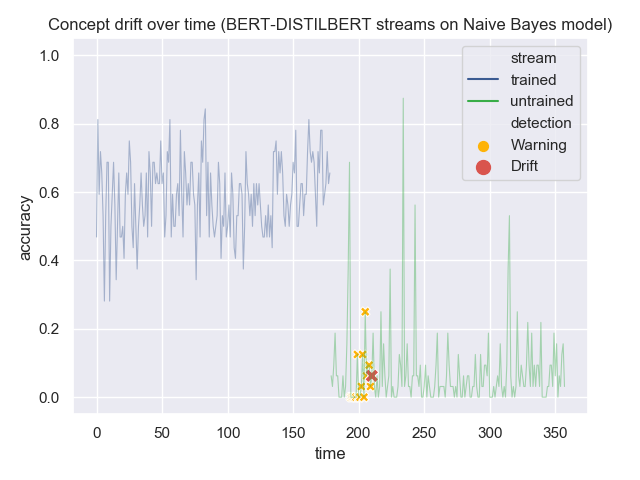
\includegraphics[width=\linewidth]{assets/detecting-change/diff_embed_nb_wos_1_BERT_DISTILBERT.png}
  \caption{Supervised change detection}
  \label{fig:nb-diff-embed-super-B-D}
\end{subfigure}%
\begin{subfigure}{.5\textwidth}
  \centering
  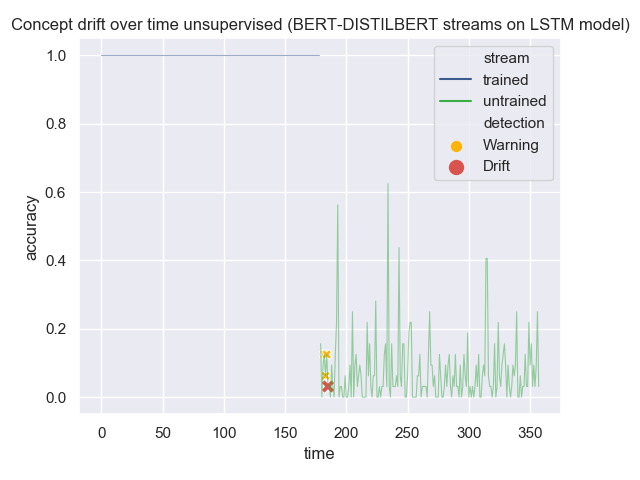
\includegraphics[width=\linewidth]{assets/detecting-change/diff_embed_nb_wos_1_BERT_DISTILBERT_unsupervised.png}
  \caption{Unsupervised change detection}
  \label{fig:nb-diff-embed-unsuper-B-D}
\end{subfigure}
\caption{Detecting change using different embeddings (BERT-DISTILBERT) in the Naive Bayes model}
\label{fig:nb-diff-embed-B-D}
\end{figure}

\begin{figure}[H]
\centering
\begin{subfigure}{.5\textwidth}
  \centering
  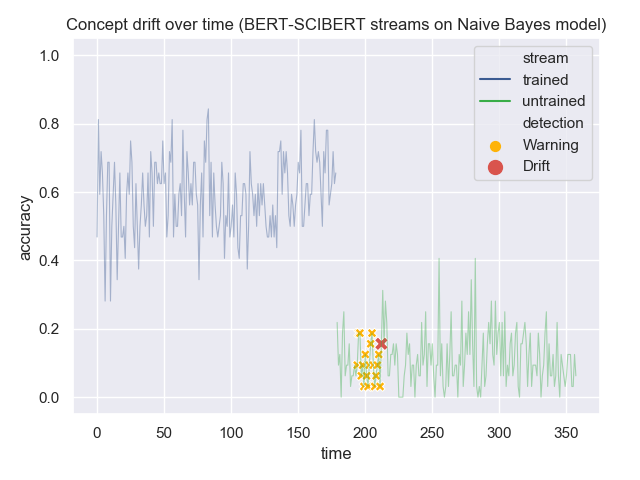
\includegraphics[width=\linewidth]{assets/detecting-change/diff_embed_nb_wos_1_BERT_SCIBERT.png}
  \caption{Supervised change detection}
  \label{fig:nb-diff-embed-super-B-S}
\end{subfigure}%
\begin{subfigure}{.5\textwidth}
  \centering
  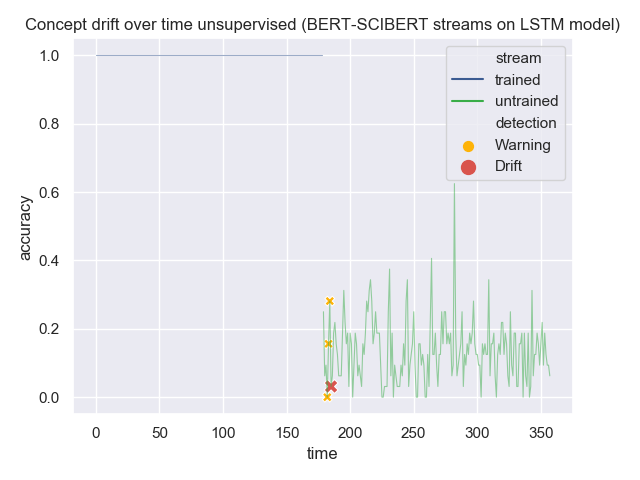
\includegraphics[width=\linewidth]{assets/detecting-change/diff_embed_nb_wos_1_BERT_SCIBERT_unsupervised.png}
  \caption{Unsupervised change detection}
  \label{fig:nb-diff-embed-unsuper-B-S}
\end{subfigure}
\caption{Detecting change using different embeddings (BERT-SCIBERT) in the Naive Bayes model}
\label{fig:nb-diff-embed-B-S}
\end{figure}

Next, we show the results of adding gradual noise to the Naive Bayes model.

\begin{figure}[H]
\centering
\begin{subfigure}{.5\textwidth}
  \centering
  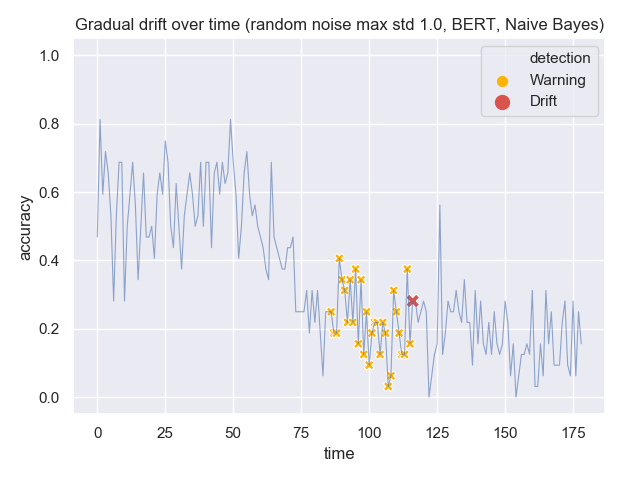
\includegraphics[width=\linewidth]{assets/detecting-change/gradual_noise_random_std_1_nb_wos_1_BERT.png}
  \caption{Gradual with std 1.0}
  \label{fig:nb-gradual-std-1}
\end{subfigure}%
\begin{subfigure}{.5\textwidth}
  \centering
  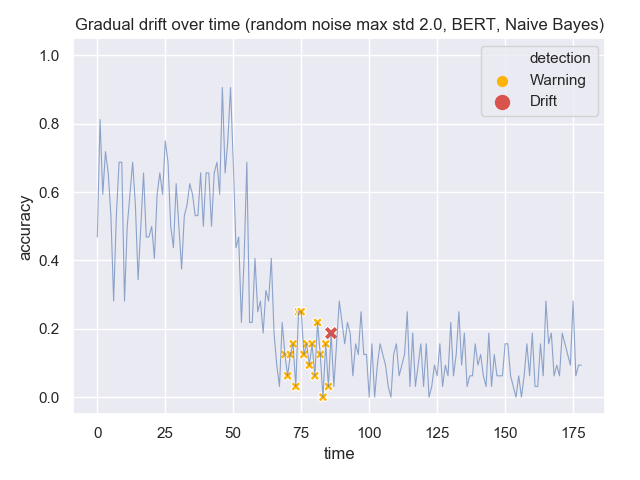
\includegraphics[width=\linewidth]{assets/detecting-change/gradual_noise_random_std_2_nb_wos_1_BERT.png}
  \caption{Gradual with std 2.0}
  \label{fig:nb-gradual-std-2}
\end{subfigure}
\begin{subfigure}{.5\textwidth}
  \centering
  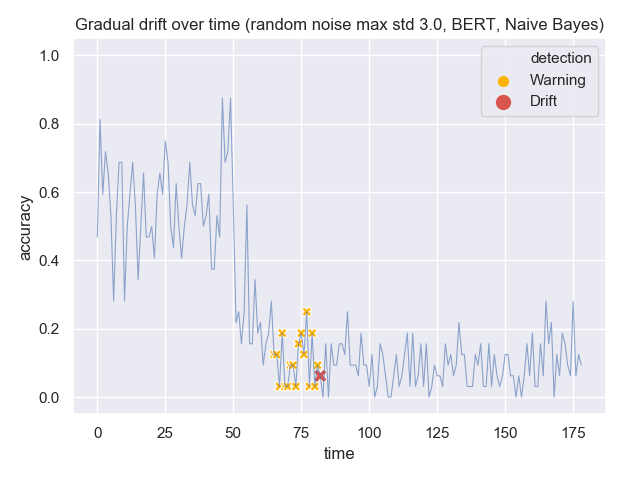
\includegraphics[width=\linewidth]{assets/detecting-change/gradual_noise_random_std_3_nb_wos_1_BERT.png}
  \caption{Gradual with std 3.0}
  \label{fig:nb-gradual-std-3}
\end{subfigure}
\caption{Detecting gradual change by adding random noise with different stds in the Naive Bayes model}
\label{fig:nb-gradual}
\end{figure}

\subsection{LSTM model}

Same things for the LSTM model.

\begin{figure}[H]
\centering
\begin{subfigure}{.5\textwidth}
  \centering
  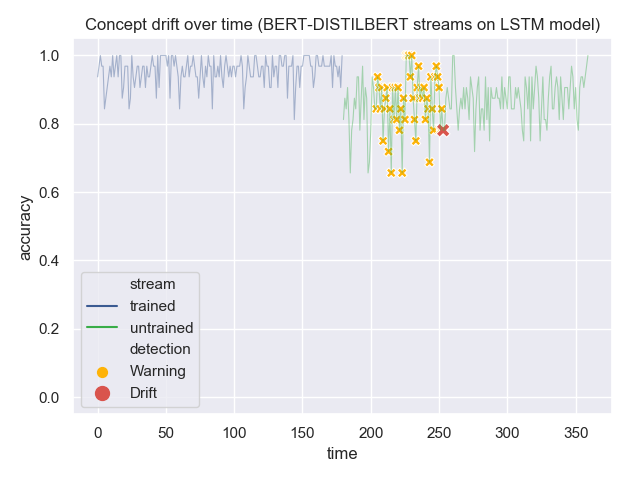
\includegraphics[width=\linewidth]{assets/detecting-change/diff_embed_lstm_wos_1_BERT_DISTILBERT.png}
  \caption{Supervised change detection}
  \label{fig:lstm-diff-embed-super-B-D}
\end{subfigure}%
\begin{subfigure}{.5\textwidth}
  \centering
  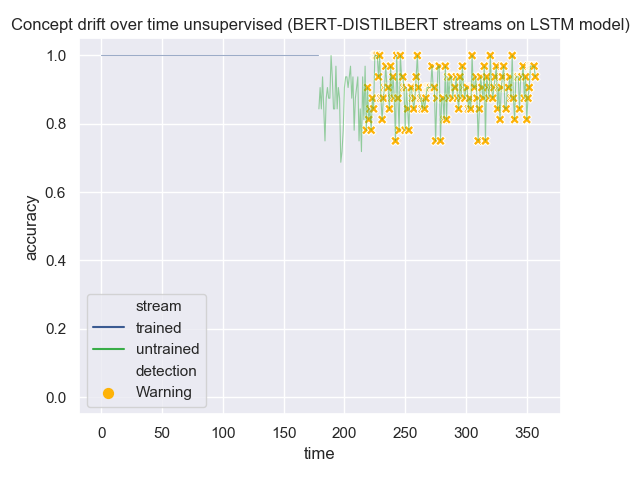
\includegraphics[width=\linewidth]{assets/detecting-change/diff_embed_lstm_wos_1_BERT_DISTILBERT_unsupervised.png}
  \caption{Unsupervised change detection}
  \label{fig:lstm-diff-embed-unsuper-B-D}
\end{subfigure}
\caption{Detecting change using different embeddings (BERT-DISTILBERT) in LSTM model}
\label{fig:lstm-diff-embed-B-D}
\end{figure}

\begin{figure}[H]
\centering
\begin{subfigure}{.5\textwidth}
  \centering
  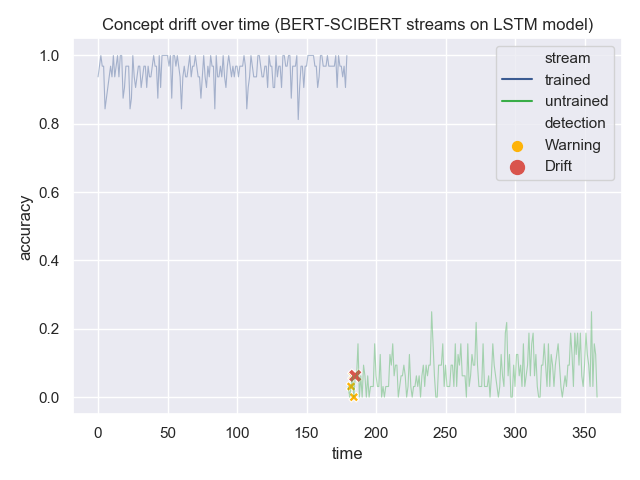
\includegraphics[width=\linewidth]{assets/detecting-change/diff_embed_lstm_wos_1_BERT_SCIBERT.png}
  \caption{Supervised change detection}
  \label{fig:lstm-diff-embed-super-B-S}
\end{subfigure}%
\begin{subfigure}{.5\textwidth}
  \centering
  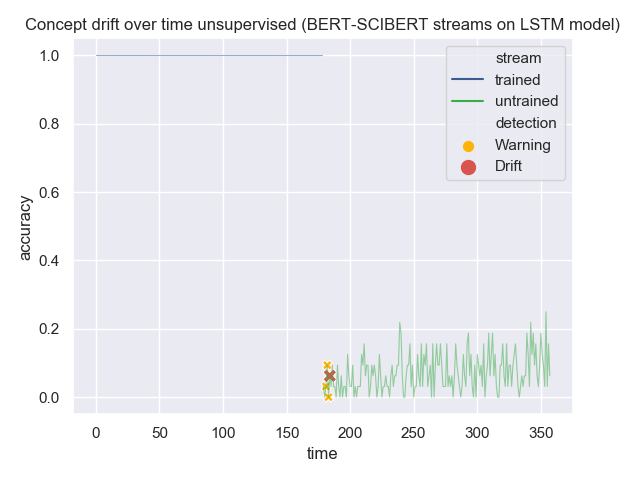
\includegraphics[width=\linewidth]{assets/detecting-change/diff_embed_lstm_wos_1_BERT_SCIBERT_unsupervised.png}
  \caption{Unsupervised change detection}
  \label{fig:lstm-diff-embed-unsuper-B-S}
\end{subfigure}
\caption{Detecting change using different embeddings (BERT-SCIBERT) in LSTM model}
\label{fig:lstm-diff-embed-B-S}
\end{figure}

Now gradual change for the LSTM model.

\begin{figure}[H]
\centering
\begin{subfigure}{.5\textwidth}
  \centering
  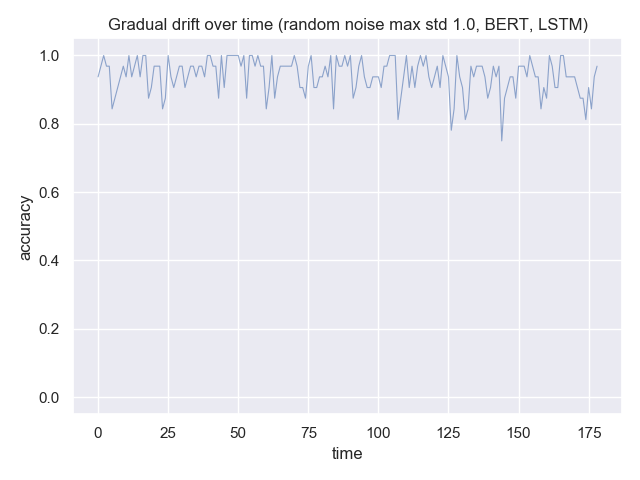
\includegraphics[width=\linewidth]{assets/detecting-change/gradual_noise_random_std_1_lstm_wos_1_BERT.png}
  \caption{Gradual with std 1.0}
  \label{fig:lstm-gradual-std-1}
\end{subfigure}%
\begin{subfigure}{.5\textwidth}
  \centering
  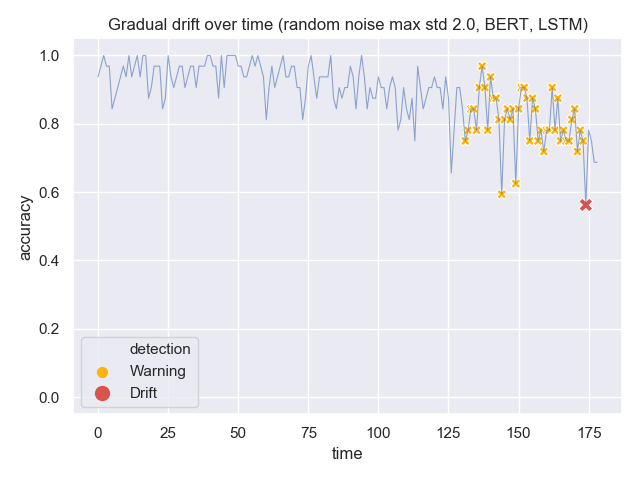
\includegraphics[width=\linewidth]{assets/detecting-change/gradual_noise_random_std_2_lstm_wos_1_BERT.png}
  \caption{Gradual with std 2.0}
  \label{fig:lstm-gradual-std-2}
\end{subfigure}
\begin{subfigure}{.5\textwidth}
  \centering
  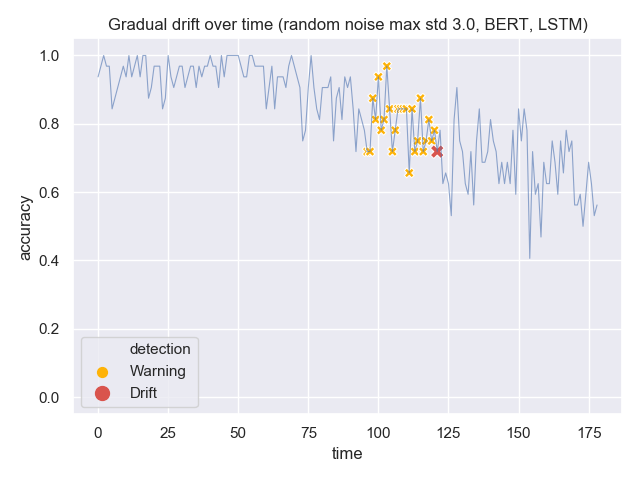
\includegraphics[width=\linewidth]{assets/detecting-change/gradual_noise_random_std_3_lstm_wos_1_BERT.png}
  \caption{Gradual with std 3.0}
  \label{fig:lstm-gradual-std-3}
\end{subfigure}
\caption{Detecting gradual change by adding random noise with different stds in the LSTM model}
\label{fig:lstm-gradual}
\end{figure}

\section{Discussion}

Main topics for discussion:
\begin{itemize}
    \item Difference in robustness between the LSTM model and the Naive Bayes model.
    \item Difference between supervised and unsupervised and how picking settings for the change detector and how we input values for accuracy to it (0.9-1) is very important and produces different results.
    \item How gradual noise affects the models
\end{itemize}

\chapter{Addressing change}

Two methods of addressing change:
\begin{itemize}
    \item For small abrupt drift or gradual drift, we can probably get away with feeding the model with a few batch and the accuracy should recover fairly fast.
    \item For big abrupt drift, one idea for adaptation is to create a mapping between the two different embedding sets.
\end{itemize}

Also mention that adaptation is useful only for the LSTM model, since the Naive Bayes is trained very fast and as such not worth performing an adaptation. Moreover, the Naive Bayes is not robust to changes in the embedding space and as such adaptation methods will probably fail.

\section{Fine Tuning}

\subsection{Experimental Setup}

Mention things like:
\begin{itemize}
    \item Using the same framework as in the detecting change section to keep things consistent.
    \item Experiments with different number of batches
    \item Also randomly select batches
\end{itemize}

\subsection{Results}

Present the results for fine tuning.

\begin{figure}[ht!]
\centering
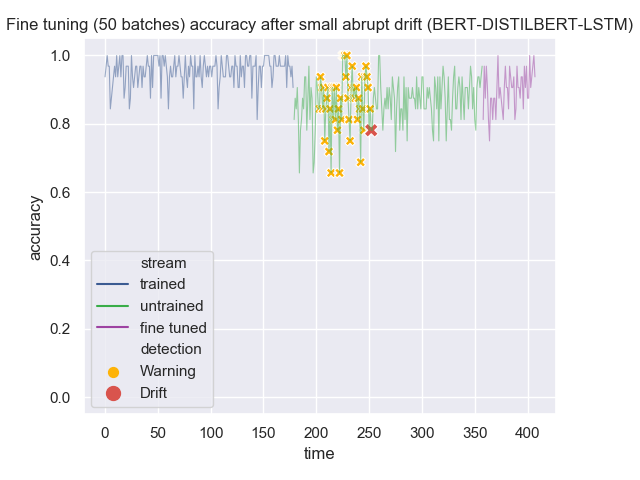
\includegraphics[width=0.8\linewidth]{assets/addressing-change/fine_tuning_lstm_wos_1_BERT_DISTILBERT_50_batches.png}
\caption{Fine tuning experiments using 50 batches}
\label{fig:fine50}
\end{figure}

\begin{figure}[ht!]
\centering
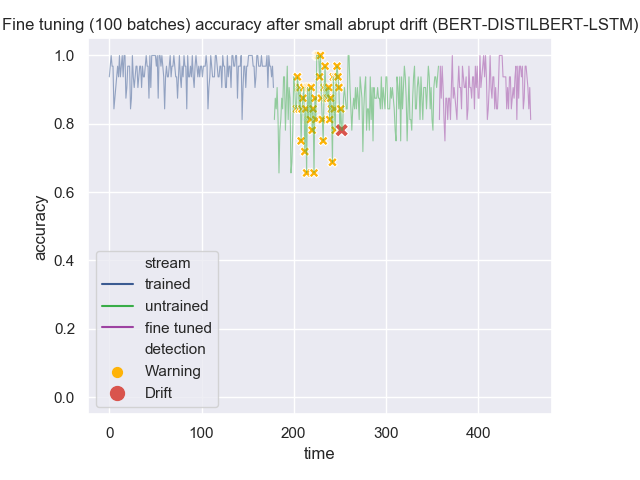
\includegraphics[width=0.8\linewidth]{assets/addressing-change/fine_tuning_lstm_wos_1_BERT_DISTILBERT_100_batches.png}
\caption{Fine tuning experiments using 100 batches}
\label{fig:fine100}
\end{figure}

TODO: also make and add results for a full epoch

TODO: might also want to create new pictures in which you run a fourth stream using already fine tuned network.

\subsection{Discussion}

Discussion on the fine tuning results.

\section{Mapping}

Maybe split this into two parts: Procrustes method and GAN method.

Explain the advantages of the Procrustes method: extremely fast, and the cons, not that reliable since it's a linear mapping. Then outline the assumption that the GAN method should be faster than retraining the whole model, and it's only worth using when that is the case.

The explain the methods used for mapping, both the Procrustes and the GAN.

Also talk about the created dataset and why it was needed.

\subsection{Experimental Setup}

Outline assumptions and decisions made in the mapping experiments.

\subsection{Results}

Show the results.

\begin{figure}[ht!]
\centering
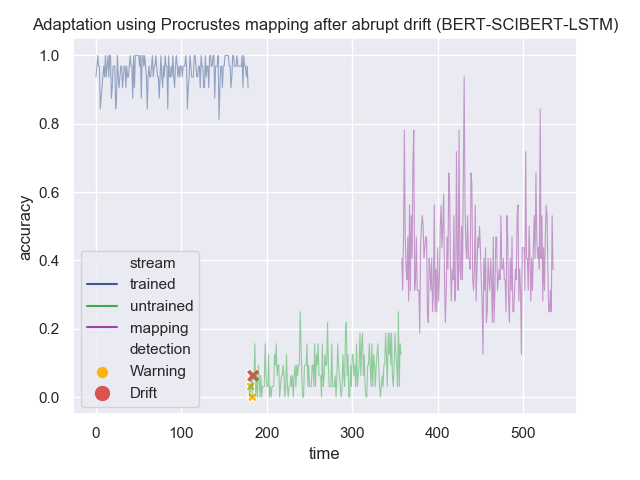
\includegraphics[width=0.8\linewidth]{assets/addressing-change/procrustes_lstm_wos_1_BERT_SCIBERT_5000_words_max.png}
\caption{Mapping using Procrustes method results using \textbf{max} embeddings aggregation in dataset}
\label{fig:proc-max}
\end{figure}

\begin{figure}[ht!]
\centering
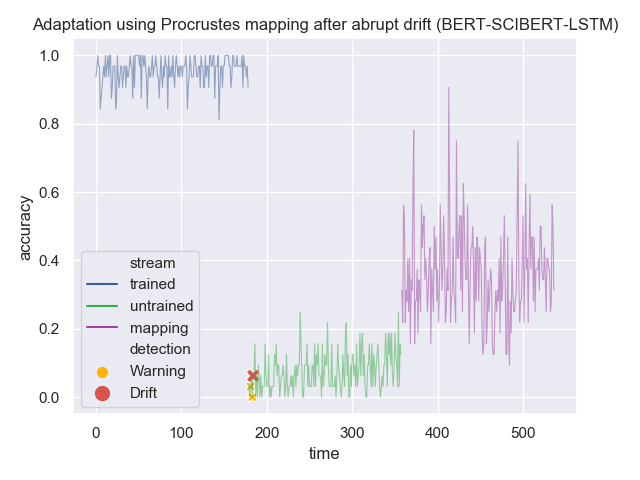
\includegraphics[width=0.8\linewidth]{assets/addressing-change/procrustes_lstm_wos_1_BERT_SCIBERT_5000_words_average.png}
\caption{Mapping using Procrustes method results using \textbf{average} embeddings aggregation in dataset}
\label{fig:proc-average}
\end{figure}

\begin{figure}[ht!]
\centering
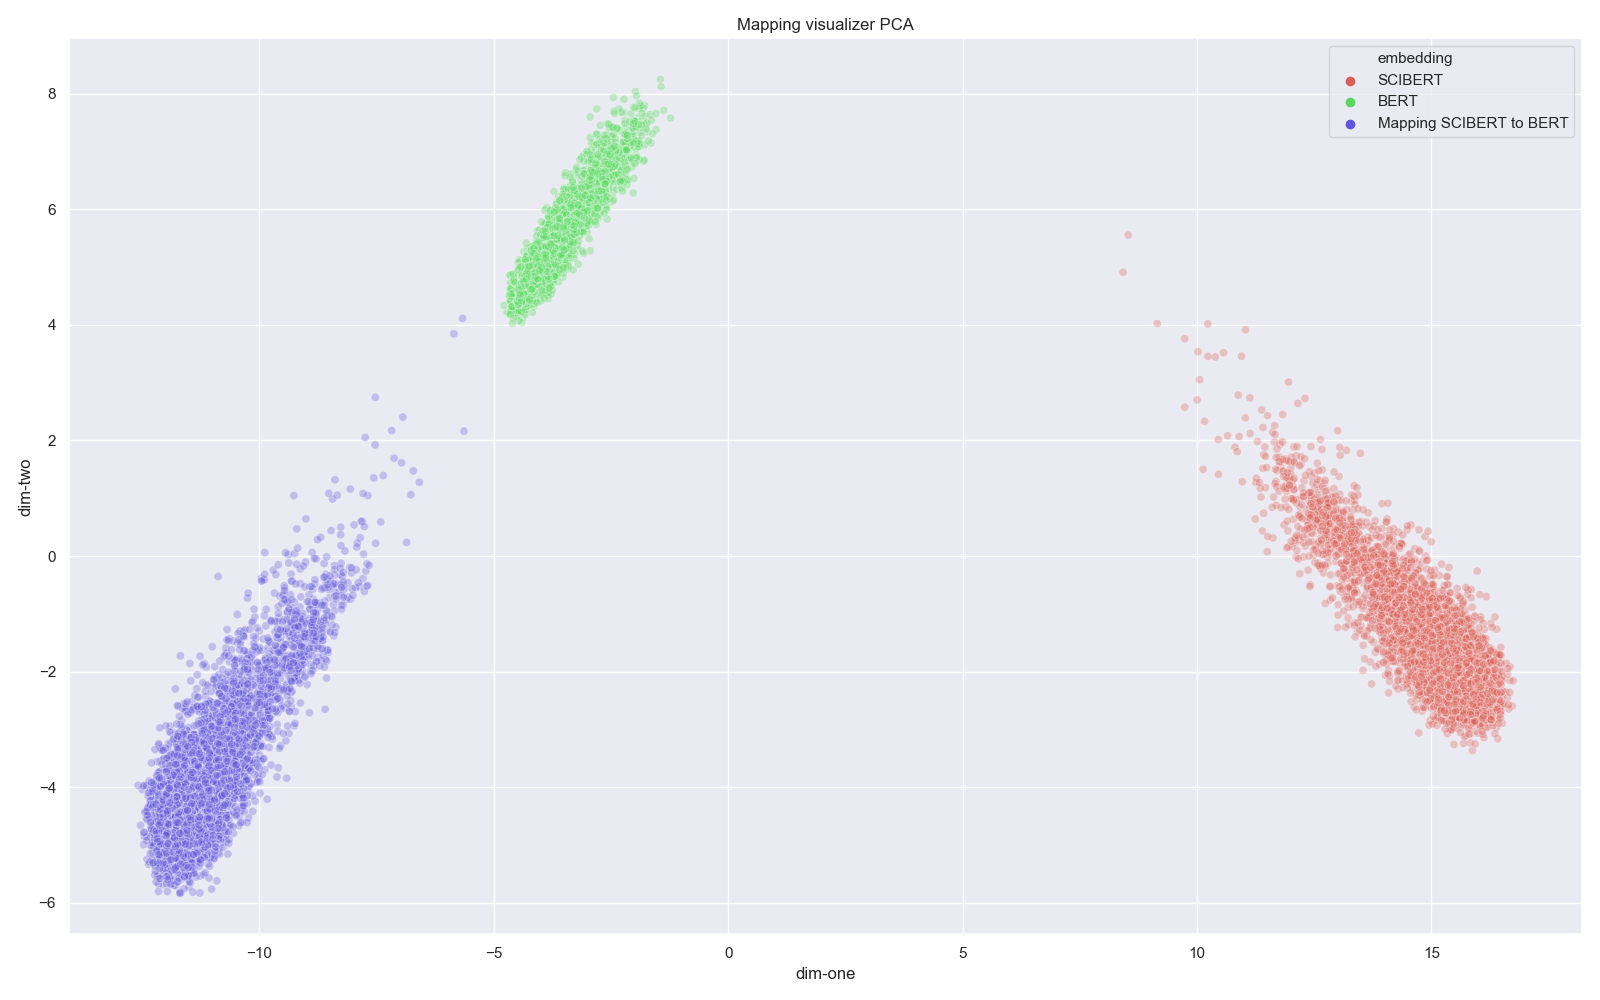
\includegraphics[width=0.8\linewidth]{assets/addressing-change/mapping_vis_pca_SCIBERT_BERT_average.png}
\caption{Embeddings spaces visualized using PCA for the Procrustes method}
\label{fig:proc-pca}
\end{figure}

\begin{figure}[ht!]
\centering
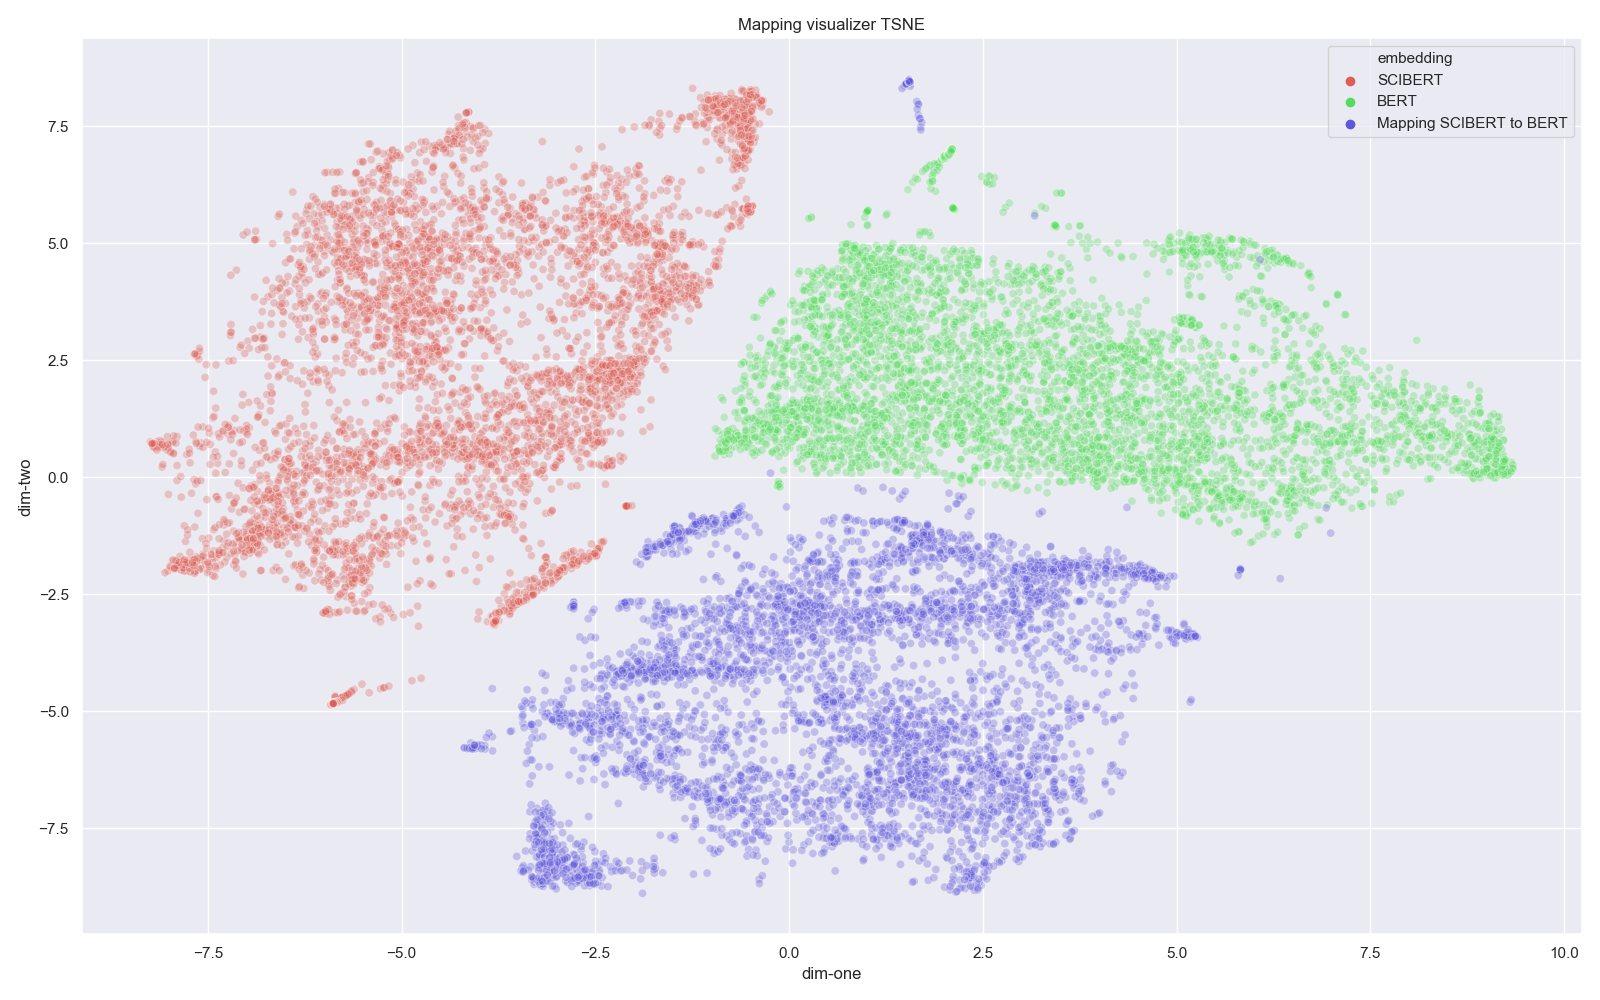
\includegraphics[width=0.8\linewidth]{assets/addressing-change/mapping_vis_tsne_SCIBERT_BERT_average.png}
\caption{Embeddings spaces visualized using t-SNE for the Procrustes method}
\label{fig:proc-tsne}
\end{figure}

\subsection{Discussion}

Discuss the results.

\chapter{Conclusion and Future Work}

\addcontentsline{toc}{chapter}{Bibliography}
\bibliographystyle{plainnat}
\bibliography{references.bib}

\end{document}

